%%%%%%%%%%%%%%%%%%%%%%%%%%%%%%%%%%%%%%%%%%%%%%%%%%%%%%%%%%%%%%%%%%%%%%
% LaTeX Template: Curriculum Vitae
%
% Source: http://www.howtotex.com/
% Feel free to distribute this template, but please keep the
% referal to HowToTeX.com.
% Date: July 2011
% 
%%%%%%%%%%%%%%%%%%%%%%%%%%%%%%%%%%%%%%%%%%%%%%%%%%%%%%%%%%%%%%%%%%%%%%
% How to use writeLaTeX: 
%
% You edit the source code here on the left, and the preview on the
% right shows you the result within a few seconds.
%
% Bookmark this page and share the URL with your co-authors. They can
% edit at the same time!
%
% You can upload figures, bibliographies, custom classes and
% styles using the files menu.
%
% If you're new to LaTeX, the wikibook is a great place to start:
% http://en.wikibooks.org/wiki/LaTeX
%
%%%%%%%%%%%%%%%%%%%%%%%%%%%%%%%%%%%%%%%%%%%%%%%%%%%%%%%%%%%%%%%%%%%%%%
\documentclass[paper=a4,fontsize=11pt]{scrartcl} % KOMA-article class
							
\usepackage[english]{babel}
\usepackage[utf8x]{inputenc}
\usepackage[protrusion=true,expansion=true]{microtype}
\usepackage{amsmath,amsfonts,amsthm}     % Math packages
\usepackage{graphicx}                    % Enable pdflatex
\usepackage[svgnames]{xcolor}            % Colors by their 'svgnames'
\usepackage{geometry}
	\textheight=700px                    % Saving trees ;-)
\usepackage{url}
\usepackage{hyperref}
%\usepackage{wrapfig}


\frenchspacing              % Better looking spacings after periods
\pagestyle{empty}           % No pagenumbers/headers/footers

%%% Custom sectioning (sectsty package)
%%% ------------------------------------------------------------
\usepackage{sectsty}

\sectionfont{%			            % Change font of \section command
	\usefont{OT1}{phv}{b}{n}%		% bch-b-n: CharterBT-Bold font
	\sectionrule{0pt}{0pt}{-5pt}{3pt}}

%%% Macros
%%% ------------------------------------------------------------
\newlength{\spacebox}
\settowidth{\spacebox}{8888888888}			% Box to align text
\newcommand{\sepspace}{\vspace*{1em}}		% Vertical space macro

\newcommand{\MyName}[1]{ % Name
		\Huge \usefont{OT1}{phv}{b}{n} \hfill #1
		\par \normalsize \normalfont}
		
\newcommand{\MySlogan}[1]{ % Slogan (optional)
		\large \usefont{OT1}{phv}{m}{n}\hfill \textit{#1}
		\par \normalsize \normalfont}

\newcommand{\NewPart}[1]{\section*{\uppercase{#1}}}

\newcommand{\PersonalEntry}[2]{
		\noindent\hangindent=2em\hangafter=0 % Indentation
		\parbox{\spacebox}{        % Box to align text
		\textit{#1}}		       % Entry name (birth, address, etc.)
		\hspace{1.5em} #2 \par}    % Entry value

\newcommand{\SkillsEntry}[2]{      % Same as \PersonalEntry
		\noindent\hangindent=2em\hangafter=0 % Indentation
		\parbox{\spacebox}{        % Box to align text
		\textit{#1}}			   % Entry name (birth, address, etc.)
		\hspace{1.5em} #2 \par}    % Entry value	
		
\newcommand{\EducationEntry}[4]{
		\noindent \textbf{#1} \hfill      % Study
		\colorbox{Black}{%
			\parbox{6em}{%
			\hfill\color{White}#2}} \par  % Duration
		\noindent \textit{#3} \par        % School
		\noindent\hangindent=2em\hangafter=0 \small #4 % Description
		\normalsize \par}

\newcommand{\WorkEntry}[4]{				  % Same as \EducationEntry
		\noindent \textbf{#1} \hfill      % Jobname
		\colorbox{Black}{\color{White}#2} \par  % Duration
		\noindent \textit{#3} \par              % Company
		\noindent\hangindent=2em\hangafter=0 \small #4 % Description
		\normalsize \par}

%%% Begin Document
%%% ------------------------------------------------------------
\begin{document}

\vspace*{-8em}
\MyName{Ph.D. Thuong Duc HOANG}
\MySlogan{
%Cosmologist \\
%\raggedleft \href{https://physics.cornell.edu/}{Department of Physics,} \\
%\raggedleft \href{https://www.cornell.edu/}{Cornell University} \\
\raggedleft {\color{blue} \href{https://hoangducthuong.github.io/}{https://hoangducthuong.github.io/} } \\
}

% you can upload a photo and include it here...
\begin{wrapfigure}[h]
	\vspace*{-7em}
		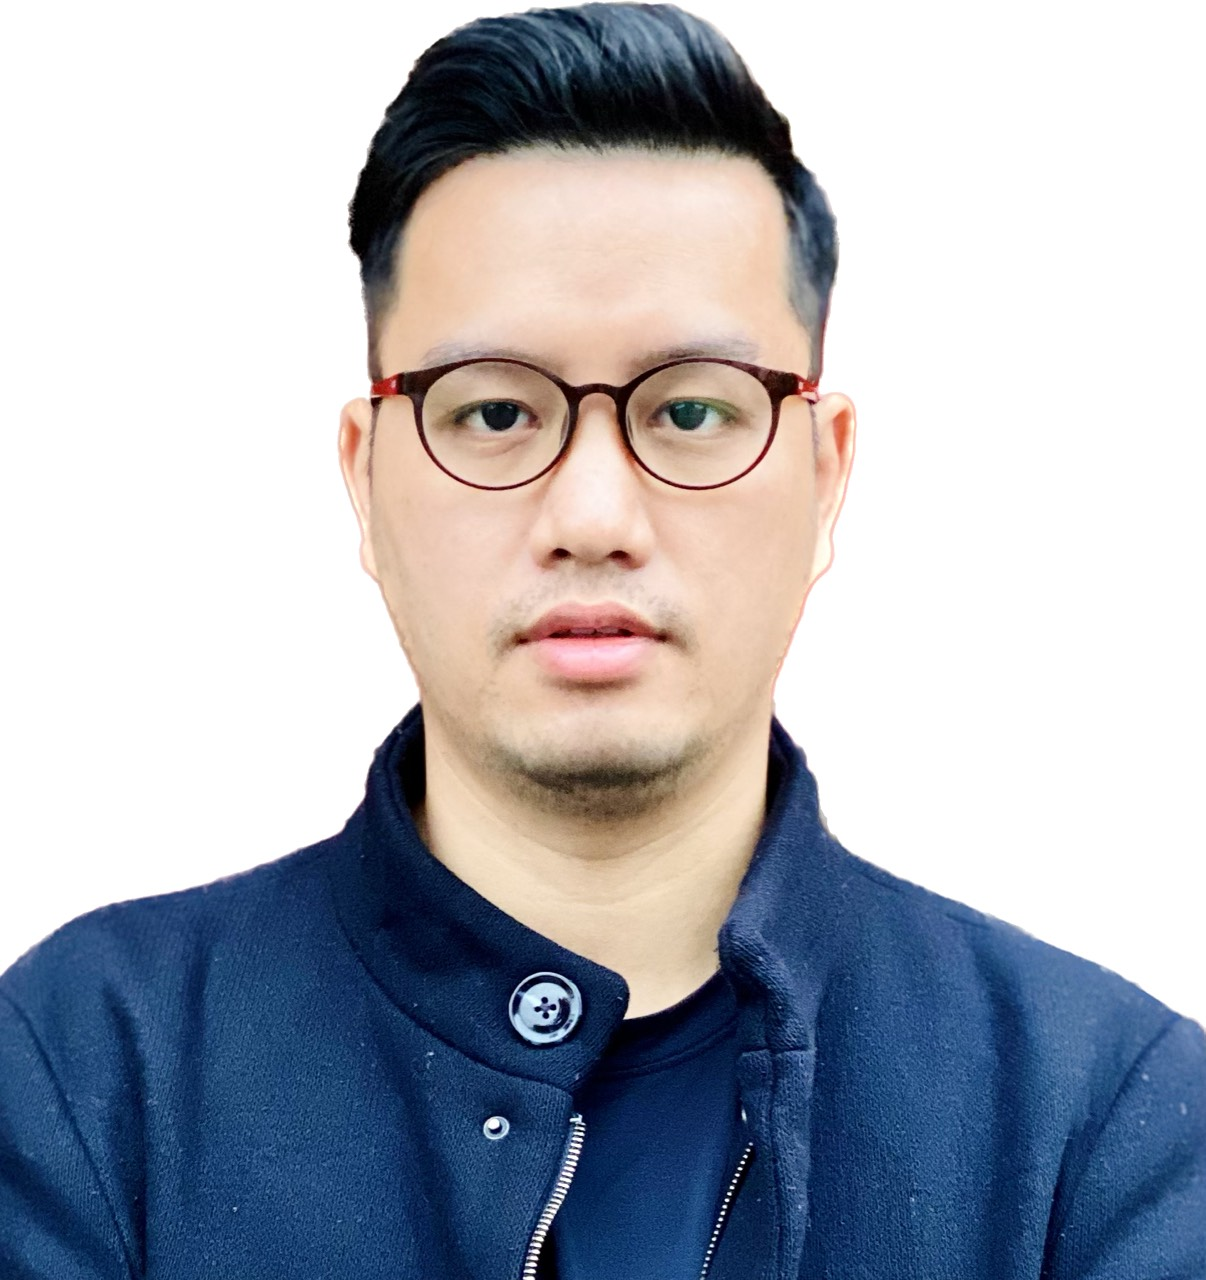
\includegraphics[width=0.2\textwidth]{Thuong.jpg}
\end{wrapfigure}
%\sepspace
\vspace*{-1.5em}
%%% Personal details
%%% ------------------------------------------------------------
\NewPart{Personal details}{}
\PersonalEntry{Degree}{ \href{https://ed560.ed.univ-paris-diderot.fr/en/the-doctoral-school/}{\textbf{Ph.D in physics of the Universe at Paris University}}   }
\PersonalEntry{Birth}{April 12, 1989}
\PersonalEntry{Nationality}{Vietnam}
\PersonalEntry{Phone}{(+84) 396158683}
%\PersonalEntry{Address}{Room 382, Physical Sciences Building, Cornell University, 245 East Avenue, Ithaca, New York, United State}
\PersonalEntry{Address}{Department of Space and Applications, University of Science and Technology of Hanoi (USTH), 18 Hoang Quoc Viet, Hanoi, Vietnam.}

%%% Education
%%% ------------------------------------------------------------
\NewPart{Education \& EXPERIENCE}{}

\EducationEntry{Lecturer/researcher}{2021-now}{ \href{https://www.usth.edu.vn}{Department of Space and Applications - University of Science and Technology of Hanoi (USTH)-Vietnam} }{Teaching modules: 
\begin{itemize}
    \item Data Analysis \& Visualization
    \item Modern cosmology
\end{itemize}
}

\sepspace


\EducationEntry{Postdoctoral scholar}{2019-2020}{ \href{https://www.cornell.edu/}{Cornell University - United States} }{ 
Testbed focal plane detectors for \href{https://simonsobservatory.org/}{the Simons Observatory} and optimization survey strategies for ground-based Cosmic Microwave Background (CMB) experiments at the Atacama desert in Chile. Supervisor: Prof. \href{https://www.classe.cornell.edu/~mdn49/}{Michael Niemack} }
\sepspace

\EducationEntry{Ph.D. in \href{http://www.apc.univ-paris7.fr/APC_CS/en}{AstroParticle and Cosmology (APC) laboratory} }{2015-2018}{Paris Diderot University-France}{
\begin{itemize}
    \item Title: Optimization of future projects for the measurement of Cosmic Microwave Background polarization. (Bandpass filters mismatch systematic effect for LiteBird satellite \& Interaction of particles with 256 superconducting Transition Edge Sensors array of QUBIC ground-based experiment). Supervisors: Assoc. Prof. Guillaume Patanchon \& Dr. Damien Prele. \href{http://theses.md.univ-paris-diderot.fr/HOANG_Duc_Thuong_1_Complete_20181217.pdf}{[{\color{blue}dissertation]} }
    \item 21-22 December 2017 Paris-France, my initiative: 1st Meeting of Young Vietnamese Community of Astronomy (YVCA), APC laboratory, Paris Diderot University. Program: {\color{blue} 
\href{https://space.usth.edu.vn/en/news/news-events/yvca-program-127.html}{https://space.usth.edu.vn/en/news/news-events/yvca-program-127.html} }
\end{itemize}
}
\sepspace

%\EducationEntry{Assistant research and teaching}{2014-2015}{Space \& Applications laboratory, University of Science and Technology of Hanoi (USTH)-(Vietnam-France University)}{
%\begin{itemize}
%	\item $13^{th}$ - $19^{th}$ 9/2015: Participation to the \href{https://ppssea.kek.jp/2015/}{4th Particle physics School in South East Asia. Speakers were Japanese professors.}
%	\item $16^{th}$ - $22^{th}$ 8/2015: Participation to the \href{https://rencontresduvietnam.org/}{Rencontres du Viet Nam} - Cosmology: 50 years after discover.
%\end{itemize}
%}
%\sepspace

\EducationEntry{\href{https://space.usth.edu.vn/}{Master Space Science \& Applications} }{2012-2014}{Double-Diploma: Observatoire de Paris and University of Science and Technology of Hanoi (USTH).}{
\begin{itemize}
    \item 3/2014 - 9/2014: Master thesis: Cosmic ray interaction with \href{https://www.cosmos.esa.int/web/planck/home}{Planck satellite} detectors for the measurement of the Cosmic Microwave Background (CMB) radiation polarization with Dr. Guillaume Patanchon at the APC laboratory.
    \item $4^{th}$ - $10^{th}$ 8/2013: Participation to the Rencontres du Viet Nam-Vietnam School of Physics on
Astrophysics and Cosmology.
    \item 6/2013 - 9/2013: (M1 thesis) Design the Software Monitoring the Operation Sequence and State of Satellite \href{https://directory.eoportal.org/web/eoportal/satellite-missions/v-w-x-y-z/vnredsat-1}{VNREDSat-1} (Vietnam Natural Resources, Environment and Disaster Monitoring Satellite) in the Space Technology Institute (STI)-Vietnam Academy of Science and Technology (VAST).
\end{itemize}
}
\sepspace

\EducationEntry{Electrical Engineering}{2007-2012}{Hanoi University of Science and Technology (HUST), School of electrical engineering, department of instrumentation and industrial informatics. Diploma: Degree of Engineer in Control and Automation Engineering.}{
\begin{itemize}
    \item 2011 - 2012: Lab work: ABB - HUST training center (teamleader). \href{https://en.wikipedia.org/wiki/ABB_Group}{ABB} is a global group in power and automation technologies.
\end{itemize}
}
\sepspace
\EducationEntry{High School: Hai Phong-Vietnam }{2004-2007}{The top pupil in math, physic and chemistry.}{}

%%% Work experience
%%% ------------------------------------------------------------
\NewPart{LANGUAGE}{}

\begin{itemize}
    \item English: Fluent
    \item French: Intermediate
\end{itemize}

%%% Skills
%%% ------------------------------------------------------------
\NewPart{SKILLS [Simulation, Instrumentation \& Data analysis]}{}

\begin{itemize}
    \item Simulation of physical processes/ Data analysis.
    \item Electronic and mechanical experiences.
\end{itemize}
\sepspace
\begin{itemize}
    \item Python (Advanced), C/C++ (intermediate), Bash shell (Basic).
    \item TOAST (Time Ordered Astrophysics Scalable Tools) (intermediate)
    \item Matlab (Intermediate).
    \item OrCAD/Altium Designer (Intermediate), Labview (Basics).
    \item \href{https://layouteditor.com/}{Layout Editor} / \href{https://www.klayout.de/}{Klayout} (Basic).
    \item \href{https://root.cern.ch/root/html/guides/users-guide/ROOTUsersGuide.html#savingreading-histograms-tofrom-a-file}{Root} (Basic).
    \item \href{https://www.solidworks.com/}{Solidwork} (Advanced), \href{https://www.3ds.com/products-services/catia/?wockw=card_content_cta_1_url%3A%22https%3A%2F%2Fblogs.3ds.com%2Fcatia%2F%22}{Catia v5/ v6} (Intermediate), \href{https://www.ansys.com/}{ANSYS} (Basic), \href{https://www.autodesk.com/}{AutoCAD} (Intermediate).
\end{itemize}
\sepspace

\begin{itemize}
    \item Latex (Advanced).
    \item Window/Linux/Mac OS (Advanced), Microsoft Office/Open Office/Keynote (Advanced).
    \item Adobe Photoshop/Lightroom/Premiere (Intermediate).
    \item WordPress/HTML/CSS (Intermediate).
\end{itemize}
\sepspace

\begin{itemize}
    \item Photography (Intermediate), caligraphy (Basic), guitar player (Intermediate).
    \item Ping-pong/badminton (Intermediate).
    \item Astronomy facebook fanpage ($\approx$ 12000 likers): {\color{blue} \url{https://www.facebook.com/thienvanhoc.org/} }
\end{itemize}
\sepspace
\begin{itemize}
    \item Google Scholar: {\color{blue} \url{https://scholar.google.com/citations?user=X6_u9x0AAAAJ&hl=en} }
\end{itemize}


%%% References
%%% ------------------------------------------------------------
\NewPart{References}{}
\sepspace
\begin{enumerate}
    \item Assoc. Prof. Guillaume PATANCHON
            \begin{itemize}
                \item Relationship: Ph.D supervisor
                \item Email: \href{mailto:guillaume.patanchon@apc.univ-paris-diderot.fr}{\color{blue} guillaume.patanchon@apc.univ-paris-diderot.fr}
                \item Phone: +33 0157276087
                \item Affiliation: AstroParticle and Cosmology (APC) laboratory - University Paris Diderot-France.
            \end{itemize}
    
    \item Prof. Michael NIEMACK
        \begin{itemize}
                \item Relationship: Postdoctoral supervisor
                \item Email: \href{mailto:niemack@cornell.edu}{\color{blue} niemack@cornell.edu}
                \item Phone: +1 607 255 0391
                \item Affiliation: Department of Physics, Cornell University, Ithaca, New York, USA.
            \end{itemize}
    \item Prof. Hirokazu ISHINO
            \begin{itemize}
                \item Relationship: Colleague
                \item Email:  \href{mailto:scishino@s.okayama-u.ac.jp}{\color{blue} scishino@s.okayama-u.ac.jp}
                \item Phone: +81-86-251-7818
                \item Affiliation: Department of Physics, Okayama University, 3-1-1 Tsushimanaka, Kita-ku, Okayama 700-8530, Japan.
            \end{itemize}
\end{enumerate}

\end{document}
